\section{Диаграмма Ганта и сетевой график изготовления продукта}

Для представления последовательности выполнения работ по разработке
методики верификации соответствия TLA+ спецификации и исходного кода
используется диаграмма Ганта. Она позволяет наглядно отобразить
продолжительность отдельных работ, временные зависимости между ними,
а также распределение задач между исполнителями проекта.

При построении календарного плана использовались результаты
декомпозиции технологического процесса, полученные в предыдущем разделе. В
отличие от полностью последовательной схемы выполнения работ, в рассматриваемом
проекте часть задач выполняется параллельно. После завершения этапа
проектирования начинается паралельная разработка необходимых частей проекта.
Это позволяет сократить общую календарную длительность проекта при сохранении
рассчитанной трудоёмкости.

Основные события и работы проекта, необходимые для построения
линейного и сетевого графиков, приведены в
таблице~\ref{tab:network_works}.

\begin{table}[h]
\centering
\caption{Основные события и работы проекта}
\label{tab:network_works}
\resizebox{\textwidth}{!}{
\begin{tabular}{|c|p{3.8cm}|p{5.8cm}|c|c|c|c|}
\hline
№ & Событие & Работа & Код & Тип & Часы & Дни \\ \hline

0 & Начало работ & -- & 0--1 & -- & 0 & 0 \\ \hline

1 & Анализ предметной области &
Анализ предметной области &
1--2 & ОН & 32 & 4 \\ \hline

2 & &
Исследование подходов &
2--3 & ОН & 40 & 5 \\ \hline

3 & &
Формирование требований &
3--4 & ОН & 24 & 3 \\ \hline

4 & Проектирование архитектуры &
Проектирование архитектуры &
4--5 & ОН & 40 & 5 \\ \hline

5 & &
Разработка взаимодействия модулей &
5--6 & ОН & 24 & 3 \\ \hline

6 & &
Выбор технологий &
6--7 & ОН & 20 & 3 \\ \hline

7 & Разработка трассроваки &
Разработка библиотеки трассировки &
7--8 & ОН & 112 & 14 \\ \hline

8 & Разработка обработки &
Подсистема агрегации трасс &
8--9 & ОН & 24 & 3 \\ \hline

9 &  &
Обработка трасс в TLA+ &
9--10 & ОН & 56 & 7 \\ \hline

10 & Тестирование и отладка &
Тестирование и отладка &
10--11 & ОН & 44 & 6 \\ \hline

11 & Подготовка документации &
Подготовка документации &
11--12 & ОН & 20 & 3 \\ \hline

12 & Документация подготовлена &
Окончание работ &
12--13 & ОН & 0 & 0 \\ \hline

\end{tabular}
}
\end{table}

На основании данных таблицы~\ref{tab:network_works} в среде Microsoft Project
была построена диаграмма Ганта (см. рис. \ref{fig:gantt}), отражающая
календарную последовательность выполнения задач, их длительность и логические
связи между ними. Диаграмма показывает, что работы по анализу предметной
области, исследованию существующих подходов и формированию требований
выполняются последовательно, поскольку каждая следующая задача опирается на
результаты предыдущей.

После завершения этапа анализа требований начинается проектирование
архитектуры, затем определяются взаимодействие модулей и используемые
технологии. Наиболее длительной работой проекта является разработка
библиотеки трассировки, поскольку именно на этом этапе реализуется
программная основа предлагаемой методики. После этого выполняются
агрегация трасс, их обработка в TLA+, тестирование и подготовка
документации.

\begin{figure}
    \centering
    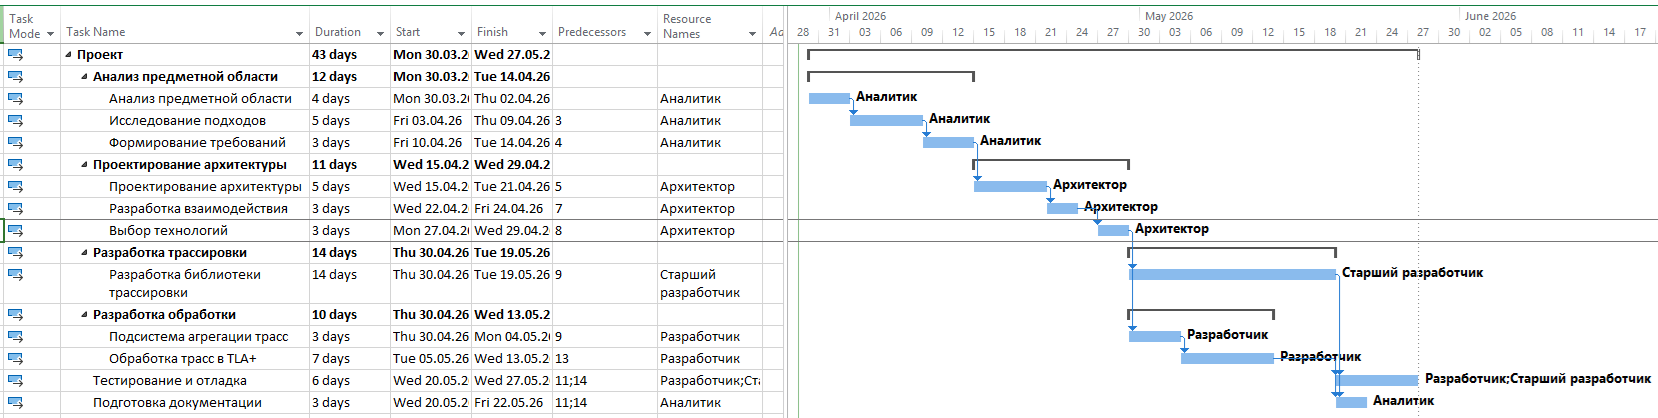
\includegraphics[width=\textwidth]{inc/gantt.png}
    \caption{Диаграмма Ганта проекта}
    \label{fig:gantt}
\end{figure}

Для оценки загрузки исполнителей был построен график использования трудовых
ресурсов (см. рис \ref{fig:resources}). Он позволяет определить, насколько
равномерно распределены задачи между участниками проекта, а также выявить
возможные перегрузки. Как видно из результатов планирования, основная нагрузка
приходится на старшего разработчика и разработчика, что обусловлено высокой
трудоёмкостью этапов реализации библиотеки трассировки, агрегации трасс и их
последующей обработки в TLA+. Аналитик активно задействован на начальном и
завершающем этапах проекта, а архитектор --- на стадии проектирования системы.

\begin{figure}
    \centering
    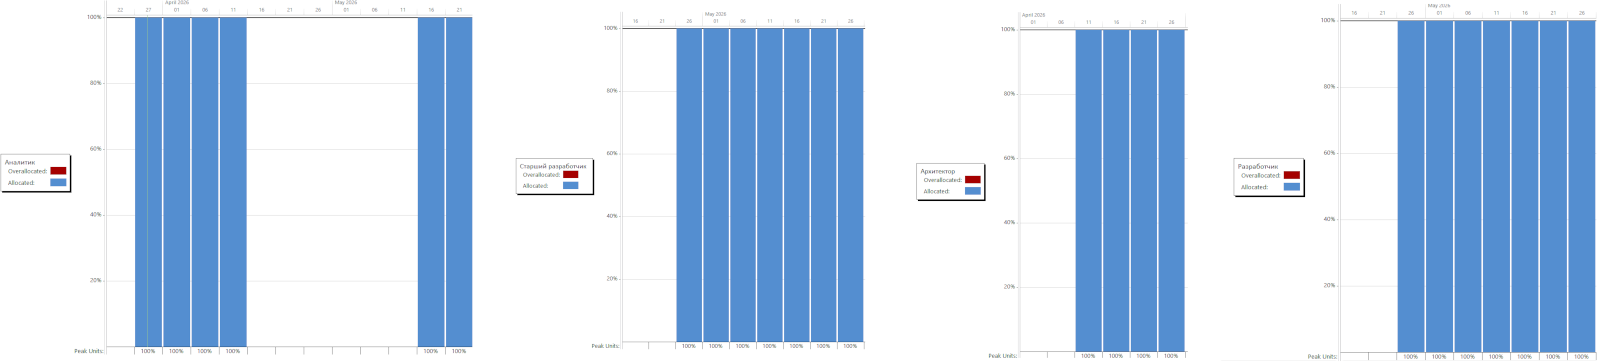
\includegraphics[width=\textwidth]{inc/labor.png}
    \caption{График использования трудовых ресурсов проекта}
    \label{fig:resources}
\end{figure}

Для более детального представления распределения работ между исполнителями была
сформирована схема распределения ресурсов по задачам (см. рис.
\ref{fig:resource_tasks}). Данная схема позволяет установить, какие именно
работы выполняются каждым участником проекта и в какие календарные периоды.
Такое представление удобно при анализе возможности параллельного выполнения
работ и оптимизации календарного плана.

\begin{figure}
    \centering
    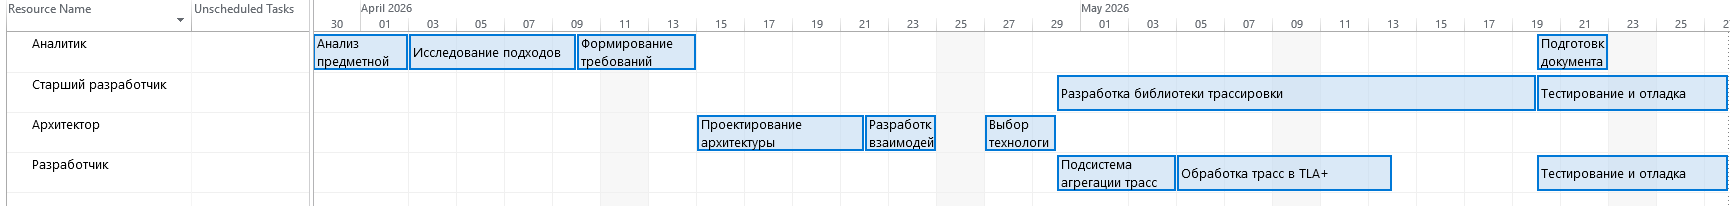
\includegraphics[width=\textwidth]{inc/resource_tasks.png}
    \caption{Визуальное представление распределения ресурсов по задачам}
    \label{fig:resource_tasks}
\end{figure}

Для анализа логической структуры проекта и выделения наиболее ответственных
работ был построен сетевой график (см. рис. \ref{fig:network}). Сетевой график
позволяет определить критический путь проекта, то есть такую последовательность
задач, задержка выполнения которой приводит к увеличению общей
продолжительности разработки.

В рассматриваемом проекте критический путь проходит через работы,
связанные с анализом предметной области, исследованием подходов,
формированием требований, проектированием архитектуры, разработкой
библиотеки трассировки, агрегацией трасс, обработкой трасс в TLA+,
тестированием и подготовкой документации. Следовательно, именно эти
работы требуют наиболее тщательного контроля сроков выполнения.

\begin{figure}
    \centering
    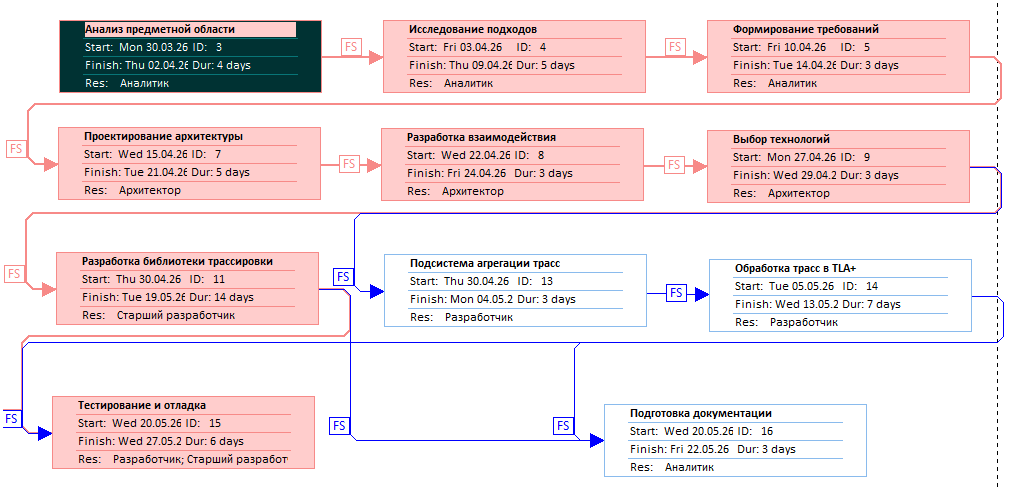
\includegraphics[width=\textwidth]{inc/network.png}
    \caption{Сетевой график проекта}
    \label{fig:network}
\end{figure}

Таким образом, построение диаграммы Ганта, графика загрузки ресурсов
и сетевого графика позволяет получить целостное представление о ходе
реализации проекта, определить временные и ресурсные ограничения, а
также выделить этапы, оказывающие наибольшее влияние на сроки
разработки продукта.

